\documentclass{article}

\usepackage{url}
\usepackage{graphicx}
\graphicspath{{figs/}}
\usepackage{subfigure}

\usepackage[utf8]{inputenc}
\usepackage[ngerman]{babel}

\usepackage{booktabs}
\usepackage{multirow}
\usepackage{pifont}
\usepackage{color}
\newcommand{\cmark}{\ding{51}}%
\newcommand{\xmark}{\ding{56}}%

\begin{document}

%don't want date printed
\date{}

\title{Verteilte Systeme Aufgabe 2 Konzept}

\author{
  Marian Triebe, Moritz Heindorf\\
  %Dept. Informatik, HAW Hamburg, Germany\\
  \{marian.triebe, moritz.heindorf\}@haw-hamburg.de
}

\maketitle

\section{Analyse der Aufgabenstellung}
Mit Hilfe von CORBA soll ein verteilter Algorithmus implementiert werden. Der verteilte Algorithmus soll einen größten gemeinsamen Teiler suchen, dabei sollen verschiedene Host Computer involviert sein auf den eine variable Anzahl an Workern erstellt werden kann. Im System gibt es einen Coordinator der die Kommunikation zwischen Client und dem restlichen System steuert. Jeder Host-PC hat zudem einen Starter Prozess laufen, welcher auf Anfrage des Coorinators Worker Prozesse starten kann.
Es soll möglich sein den Systemzustand zu erfassen. Dazu muss der wird in sequentiellen Abständen eine Terminierungserfassung gestartet, dazu werden im System Marker verschickt und ausgewertet. Die letzte Komponente im System ist der Monitor, welcher den Systemzustand ausgeben kann, dieses Programm ist bereits gestellt.

\section{Aufbau der Programme}
Es sind 4 Programme zu entwerfen (Client, Starter, Coordinator, Worker). Wir haben diese als Klassendiagramm dargestellt, da jedes Programm nur eine CORBA Entität repräsentiert.\\
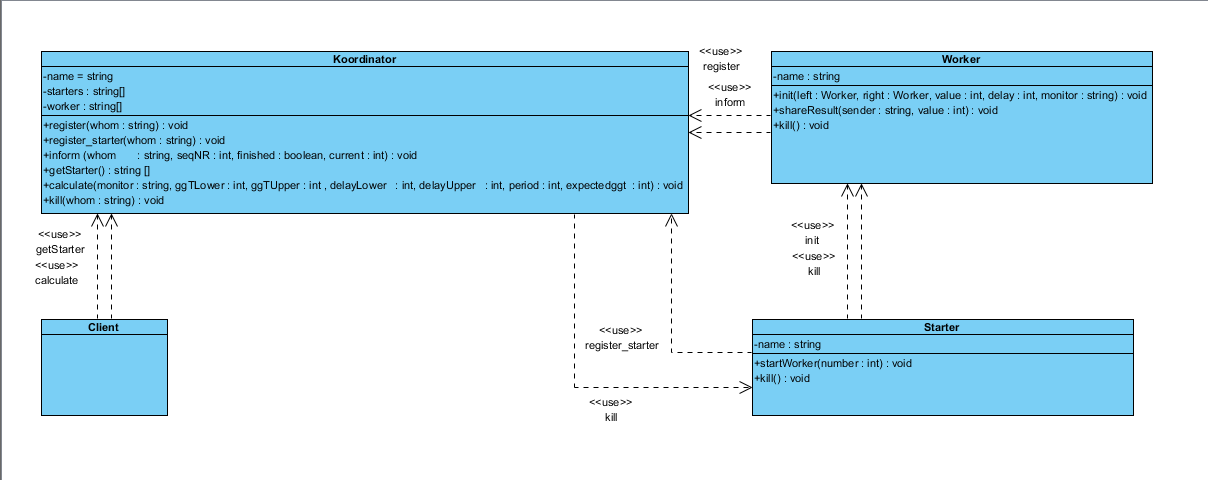
\includegraphics[scale=.40]{Documents/ClassDiagram}\\
Das Klassendiagramm ist unvollständig und besitzt noch nicht alle notwendigen Member, jedoch sind schon alle Funktionsaufrufe die wir durch CORBA Aufrufbar machen wollen vorhanden. Die IDL Files sind ebenfalls schon entstanden und decken sich mit diesem Diagramm.

\section{Kommunikationsablauf}
In diesem Sequenzdiagramm beschreiben wir den Ablauf beim starten einer neuen Berechnung durch den Benutzer.\\
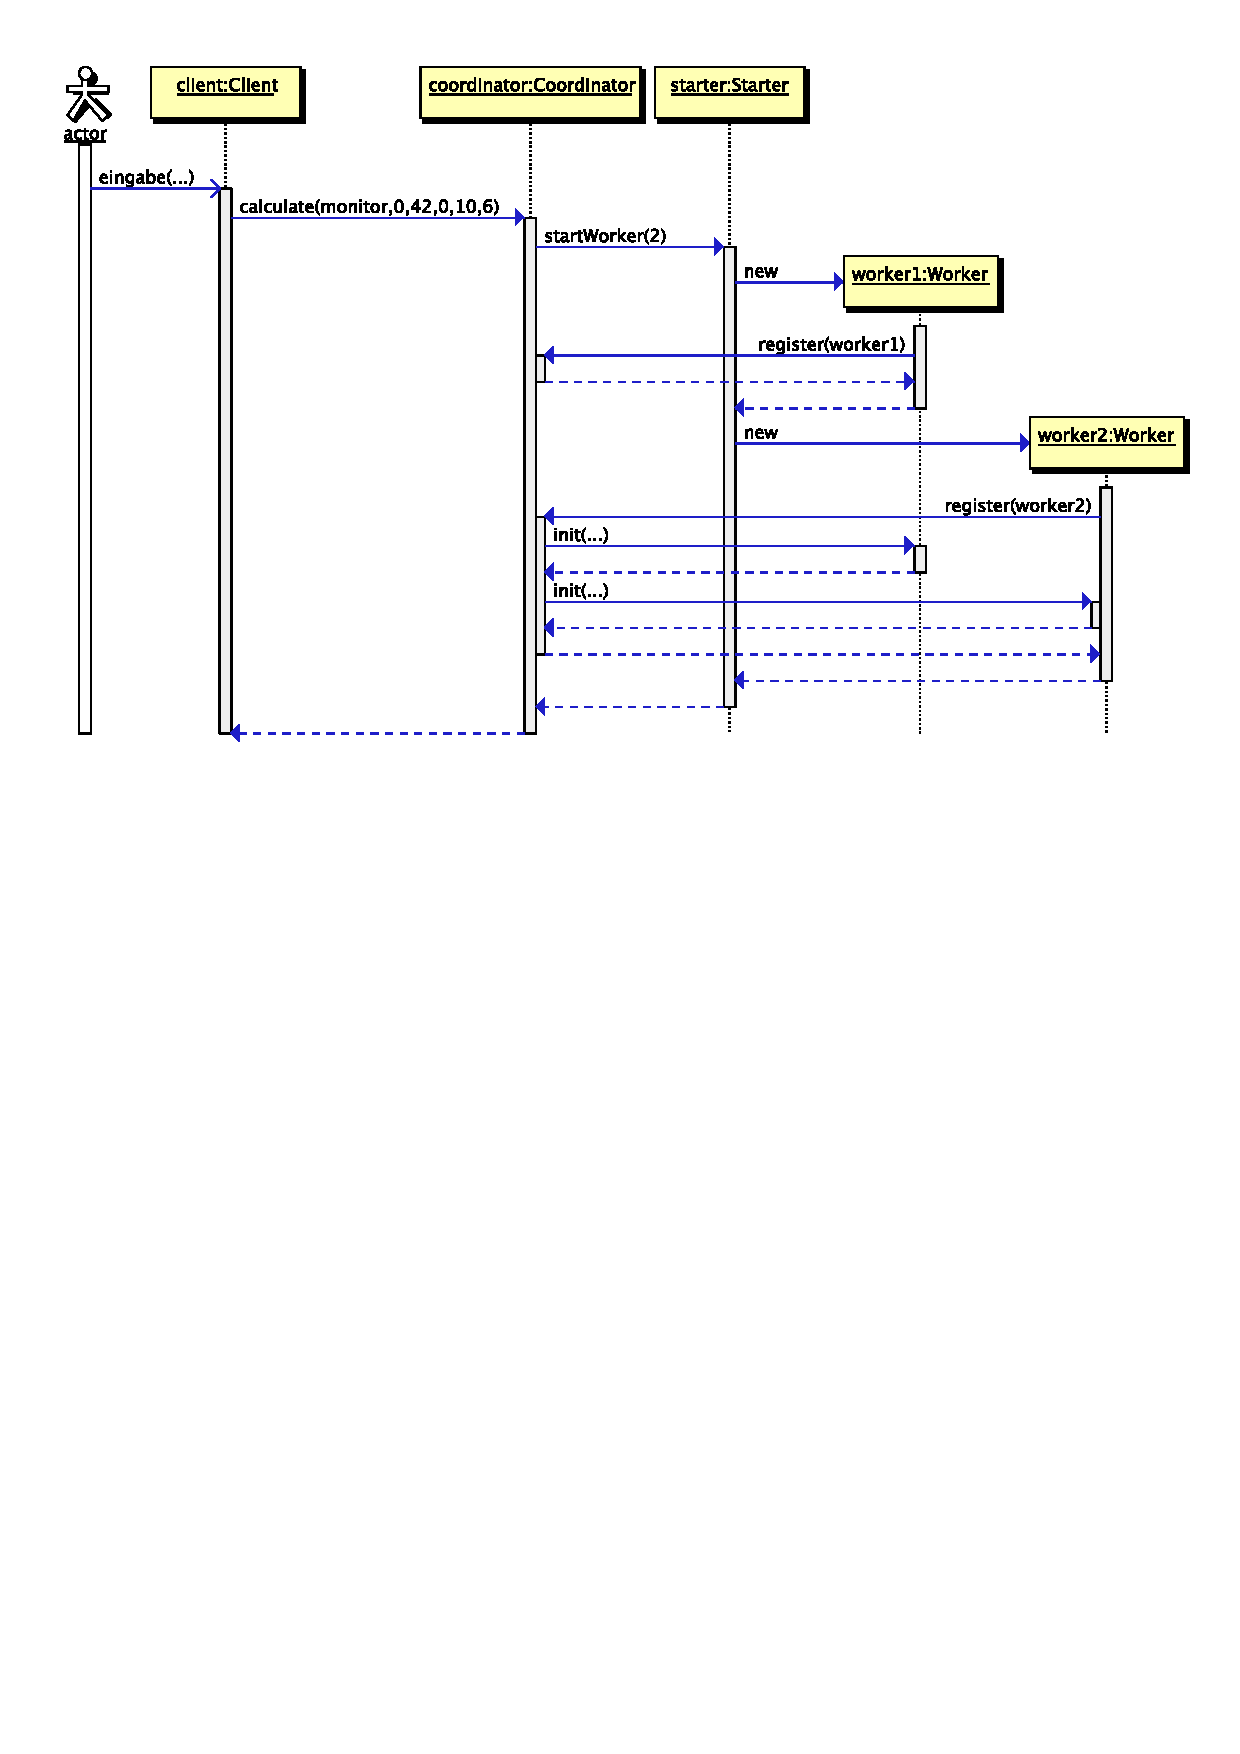
\includegraphics[scale=.6]{spawn_workers}\\
Wie in der Grafik zu sehen, werden die Daten vom Client an den Coordinator gereicht, dieser sendet dann eine \textit{startWorker()} Anfrage an den spezifizierten Starter, dieser wiedrum startet die gewünschte Anzahl an Worker. Die Worker melden sich nun beim Coordinator an.

\section{Mögliche Probleme}
\begin{itemize}
	\item Verschachtelte Monitor Aufrufe die zu Deadlock führen
	\item Thread sichere Programmierung
	\item Bindung von Workern zu Startern
	\item Terminierung von Workern, die Nachbar Worker bekommen dies nicht richtig mit
	\item Wie soll reagiert werden wenn ein Nachbar ausfällt?
	\item Starten eines neuen Prozesses aus einem Java Prozess?
\end{itemize}
\end{document}
